%%%%%%%%%%%%%%%%%%%%%%%%%%%%%%%%%%%%%%%%%
% Beamer Presentation
% LaTeX Template
% Version 1.0 (10/11/12)
%
% This template has been downloaded from:
% http://www.LaTeXTemplates.com
%
% License:
% CC BY-NC-SA 3.0 (http://creativecommons.org/licenses/by-nc-sa/3.0/)
%
%%%%%%%%%%%%%%%%%%%%%%%%%%%%%%%%%%%%%%%%%

%----------------------------------------------------------------------------------------
%	PACKAGES AND THEMES
%----------------------------------------------------------------------------------------

\documentclass{beamer}

\mode<presentation> {

% The Beamer class comes with a number of default slide themes
% which change the colors and layouts of slides. Below this is a list
% of all the themes, uncomment each in turn to see what they look like.

%\usetheme{default}
%\usetheme{AnnArbor}
%\usetheme{Antibes}
%\usetheme{Bergen}
%\usetheme{Berkeley}
\usetheme{Berlin}
%\usetheme{Boadilla}
%\usetheme{CambridgeUS}
%\usetheme{Copenhagen}
%\usetheme{Darmstadt}
%\usetheme{Dresden}
%\usetheme{Frankfurt}
%\usetheme{Goettingen}
%\usetheme{Hannover}
%\usetheme{Ilmenau}
%\usetheme{JuanLesPins}
%\usetheme{Luebeck}
%\usetheme{Madrid}
%\usetheme{Malmoe}
%\usetheme{Marburg}
%\usetheme{Montpellier}
%\usetheme{PaloAlto}
%\usetheme{Pittsburgh}
%\usetheme{Rochester}
%\usetheme{Singapore}
%\usetheme{Szeged}
%\usetheme{Warsaw}

% As well as themes, the Beamer class has a number of color themes
% for any slide theme. Uncomment each of these in turn to see how it
% changes the colors of your current slide theme.

%\usecolortheme{albatross}
%\usecolortheme{beaver}
%\usecolortheme{beetle}
%\usecolortheme{crane}
%\usecolortheme{dolphin}
%\usecolortheme{dove}
%\usecolortheme{fly}
%\usecolortheme{lily}
%\usecolortheme{orchid}
%\usecolortheme{rose}
%\usecolortheme{seagull}
\usecolortheme{seahorse}
%\usecolortheme{whale}
%\usecolortheme{wolverine}

%\setbeamertemplate{footline} % To remove the footer line in all slides uncomment this line
%\setbeamertemplate{footline}[page number] % To replace the footer line in all slides with a simple slide count uncomment this line

%\setbeamertemplate{navigation symbols}{} % To remove the navigation symbols from the bottom of all slides uncomment this line
}

\usepackage{graphicx} % Allows including images
\usepackage{booktabs} % Allows the use of \toprule, \midrule and \bottomrule in tables

%----------------------------------------------------------------------------------------
%	TITLE PAGE
%----------------------------------------------------------------------------------------

\title[ARM]{ARM Processors} % The short title appears at the bottom of every slide, the full title is only on the title page

\author{Saurabh, Tushar, Nitesh, Rohan, Paritosh} % Your name
\institute[VIT U] % Your institution as it will appear on the bottom of every slide, may be shorthand to save space
{
VIT University\\ % Your institution for the title page
% Your email address
}
% Date, can be changed to a custom date

\begin{document}

\begin{frame}
\titlepage % Print the title page as the first slide
\end{frame}

\begin{frame}
\frametitle{Overview} % Table of contents slide, comment this block out to remove it
\tableofcontents % Throughout your presentation, if you choose to use \section{} and \subsection{} commands, these will automatically be printed on this slide as an overview of your presentation
\end{frame}

%----------------------------------------------------------------------------------------
%	PRESENTATION SLIDES
%----------------------------------------------------------------------------------------

%------------------------------------------------
\section{Introduction} % Sections can be created in order to organize your presentation into discrete blocks, all sections and subsections are automatically printed in the table of contents as an overview of the talk
%------------------------------------------------

\subsection{What is ARM ?} % A subsection can be created just before a set of slides with a common theme to further break down your presentation into chunks

\begin{frame}
\frametitle{ARM: Advanced RISC Machines }
\begin{columns}[c] % The "c" option specifies centered vertical alignment while the "t" option is used for top vertical alignment

\column{.45\textwidth} % Left column and width
\textbf{Origins}
\begin{itemize}
\item Originated in England in 1984 as Acorn RISC Machines.
\item Used mostly for educational systems.
\item In 1990, the research section of Acorn separated from the parent company and formed: ARM Ltd.
\end{itemize}

\column{.5\textwidth} % Right column and width
\begin{figure}
\includegraphics[width=0.8\linewidth]{arm_originate.png}
\caption{England}
\end{figure}

\end{columns}

\end{frame}

%------------------------------------------------

\begin{frame}
\frametitle{RISC Machines ?}
Basically, a simpler and configurable design for small-scale systems.
\begin{itemize}
\item RISC stands for "Reduced Instruction Set Computer"
\item Comparision with CISC (Complex Instruction Set Computer)
\begin{itemize}
\item  Fixed 32-bit instruction size instead of variable.
\item Larger Register Bank of 32-bit Registers.
\item Easier to prototype and put together.
\end{itemize}
\end{itemize}

\end{frame}

%------------------------------------------------
\subsection{Why ARM ?}
\begin{frame}
\frametitle{Why is ARM special}
\begin{columns}[c] % The "c" option specifies centered vertical alignment while the "t" option is used for top vertical alignment

\column{.45\textwidth} % Left column and width
\textbf{Selling Points}
\begin{itemize}
\item Best MIPS (Million Instructions Per Second) to Watts ratio
\item Best MIPS to \$ ratio in the industry.
\item The smallest CPU die size.
\item Highly Customizable and Flexible.
\end{itemize}

\column{.45\textwidth} % Right column and width
\begin{figure}
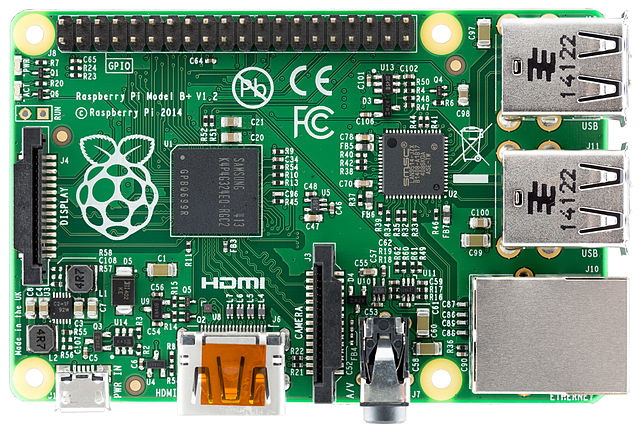
\includegraphics[width=0.8\linewidth]{Raspberry_Pi.jpg}
\caption{A Raspberry Pi.}
\end{figure}

\end{columns}
\end{frame}

%------------------------------------------------

\begin{frame}
\frametitle{Market Share}
The low power consumption of ARM processors has made them very popular: over 50 billion ARM processors have been produced as of 2014.
\begin{figure}
\includegraphics[width=0.45\linewidth]{arm_devices.jpg}
\caption{ARM-based chips are found in nearly 60 percent of the world’s mobile devices.}
\end{figure}
\end{frame}

%------------------------------------------------
\section{Architecture}
%------------------------------------------------
\subsection{Data and Instruction Storage}
\begin{frame}
\frametitle{Data Sizes and Instruction Sets}
\begin{itemize}
\item When used in relation to ARM
  \begin{itemize}
  \item \textbf{Halfword} - 16 bits.
  \item \textbf{Word} - 32 bits.
  \item \textbf{Doubleword} - 64 bits.
  \end{itemize}
\item Most ARMs implement two instruction sets
  \begin{itemize}
  \item 32 bit ARM instruction set
  \item 16 bit Thumb instruction set
  \end{itemize}
\item Jazelle-DBX cores can also execute Java bytecode
\end{itemize}
\end{frame}

%------------------------------------------------
\subsection{Processor Modes}
\begin{frame}
\frametitle{Processor Modes}
\begin{itemize}
\item The ARM has seven basic operating modes
\item Each mode has its own stack and a different set of registers
\item Some operations can only be carried out in a privileged mode
\end{itemize}
 % Right column and width
\begin{figure}
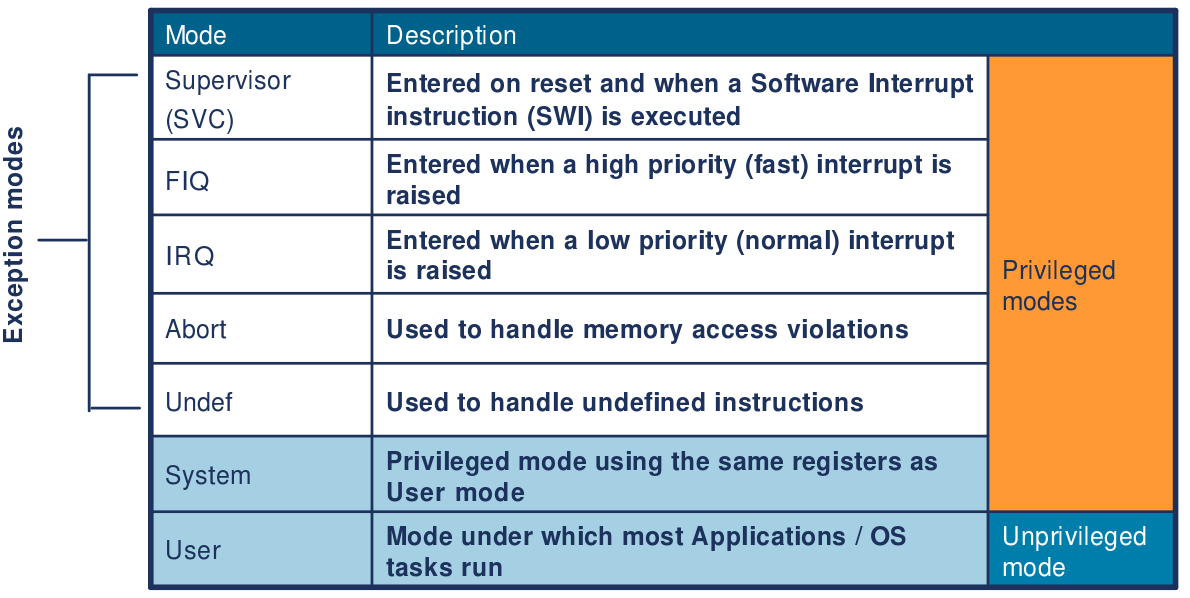
\includegraphics[width=0.8\linewidth]{ARM_modes.png}

\end{figure}
\end{frame}


%------------------------------------------------
\subsection{Register Set}


\begin{frame}% Need to use the fragile option when verbatim is used in the slide
\frametitle{Register Set}
\begin{figure}
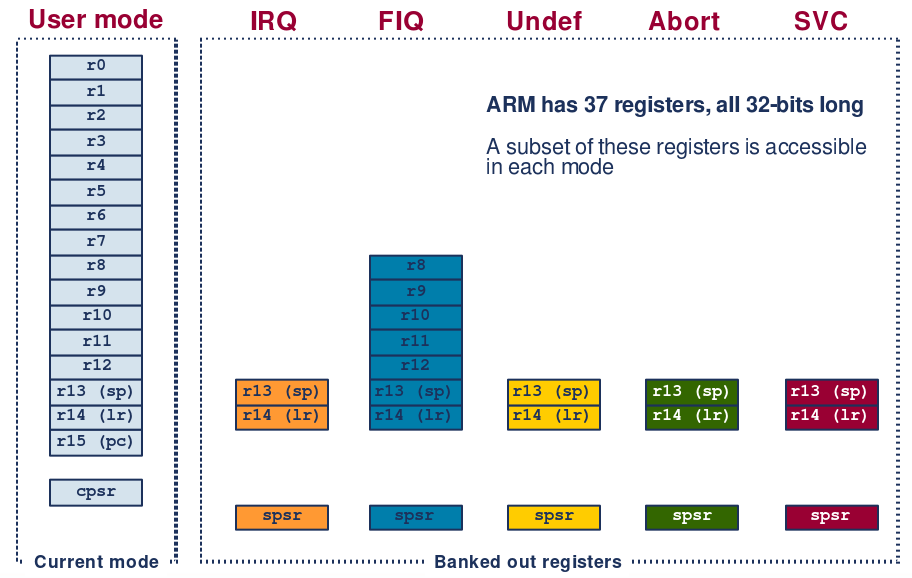
\includegraphics[width=0.8\linewidth]{ARM_register.png}
\caption{ARM Register Set.}
\end{figure}
\end{frame}



%------------------------------------------------

%------------------------------------------------
\section{Instruction Sets}
%------------------------------------------------
\subsection{Instruction Sets}

\begin{frame}
\frametitle{ARM Instruction Set}
All instructions are 32 bit long.
Examples

\begin{table}
\begin{tabular}{l l l}
\toprule
\textbf{Instruction} & \textbf{Type} & \textbf{Comment}\\
\midrule
\texttt{sub r0, r1, \#5} & data processing  & r0 = r1 -5 \\
\texttt{B <Label>} & branching & jump (+/- 32MB) \\
\texttt{LDR r0 [r1]} & memory access & load word at address r1 into r0 \\
\bottomrule
\end{tabular}
\caption{Examples of ARM instructions}
\end{table}


\end{frame}

%------------------------------------------------


\begin{frame}
\frametitle{Thumb Instruction Set}

\begin{itemize}
\item 16 bit instruction set.
\begin{itemize}
\item Optimized for code density from C code (~65\% ARM code size)
\item Improved performance for narrow memory.
\item Subset of functionality of ARM instruction set.
\end{itemize}
\item Not a "regular" instruction set.
\begin{itemize}
\item Constraints are not generally consistent.
\item Targeted at compiler generation, not hand-coding.
\end{itemize}
\end{itemize}
\end{frame}

%------------------------------------------------


\begin{frame}
\frametitle{Thumb-2 Instruction Set}

\begin{itemize}
\item A major extension to the Thumb Instruction Set
\begin{itemize}
\item Adds 32-bit instructions to implement almost all of the ARM functionality
\item Retains the complete 16-bit Thumb instruction set
\end{itemize}
\item Design objective: ARM performance with Thumb code density
\begin{itemize}
\item No switching between states.
\item The Compiler automatically selects mix of 16 and 32 bit instructions.
\end{itemize}
\end{itemize}
\end{frame}

\subsection{Comparision}
\begin{frame}% Need to use the fragile option when verbatim is used in the slide
\frametitle{Comparision}
\begin{figure}
\includegraphics[width=0.8\linewidth]{ARM_compare.png}
\end{figure}
\end{frame}



\section{Processors}
\subsection{List of ARM Processors}
\begin{frame}
\frametitle{ARM Processors}

\begin{itemize}
\item ARM1
\begin{itemize}
\item The first ARM processor
\item Used for evaluation systems, mainly a prototype
\end{itemize}
\item ARM2
\begin{itemize}
\item 27 registers, 16 accessible at one time.
\item 8 MHz, 4 Million instructions per second
\end{itemize}

\item ARM3
\begin{itemize}
\item First integrated memory cache.
\item Coprocessor interface added.
\item 25 MHz, 12 Million instructions per second
\end{itemize}

\end{itemize}
\end{frame}

%---
\begin{frame}
\frametitle{ARM Processors}

\begin{itemize}

\item ARM4 \& ARM5
\begin{itemize}
\item Never made.
\item Numbering scheme changed due to shift from Acorn to ARM ltd.
\end{itemize}

\item ARM6
\begin{itemize}
\item First to have 32 bit addressing capability.
\item 31 registers, 36,000 transistors
\item 33 MHz, 36 Million instructions per second
\end{itemize}


\item ARM7
\begin{itemize}
\item Functionally identical to ARM6.
\item 26-bit addressing support dropped.
\item 40 MHz, 4 Million instructions per second
\end{itemize}

\end{itemize}
\end{frame}

%---

\begin{frame}
\frametitle{ARM Processors}

\begin{itemize}

\item ARM8
\begin{itemize}
\item 5-stage pipeline.
\item 80 MHz, 80 Million instructions per second
\end{itemize}

\item StrongARM
\begin{itemize}
\item Developed by ARM ltd in conjunction with Digital.
\item 5-stage pipeline.
\item 200 MHz, 230 Million instructions per second
\end{itemize}

\item ARM9
\begin{itemize}
\item 180 MHz, 200 Million instructions per second
\end{itemize}

\end{itemize}
\end{frame}

%---
\begin{frame}
\frametitle{ARM Processors}

\begin{itemize}


\item ARM10
\begin{itemize}
\item Developed by ARM ltd in conjunction with Digital .
\item 300 MHz, 400 Million instructions per second
\end{itemize}
\end{itemize}
\end{frame}

\subsection{Cortex}
\begin{frame}
\frametitle{Cortex}


The ARM series were succeeded by the Cortex series of processors
\begin{itemize}

\item Cortex-M
\item Cortex-R
\item Cortex-A (32-bit)
\item Cortex-A (64-bit)

\end{itemize}
\end{frame}


%------------------------------------------------


%------------------------------------------------
\begin{frame}
\Huge{\centerline{The End}}
\end{frame}

%----------------------------------------------------------------------------------------

\end{document}
